\documentclass[
    11pt, % Set the default font size, options include: 8pt, 9pt, 10pt, 11pt, 12pt, 14pt, 17pt, 20pt
    %
    aspectratio=169, % Uncomment to set the aspect ratio to a 16:9 ratio which matches the aspect ratio of 1080p and 4K screens and projectors
]{beamer}
\usepackage{hyperref}
%\graphicspath{{Images/}{./}} % Specifies where to look for included images (trailing slash required)
\usepackage{booktabs} % Allows the use of \toprule, \midrule and \bottomrule for better rules in tables

%\usepackage{appendixnumberbeamer} %If you want a separate slide counter for your appendix

%%% Customize Theme %%%%%%%%%%%%%%%%%%%%%%
\usetheme{Madrid} % You can use other themes too, but this changes many things. I've found Madrid to be the best for this color scheme

%fg = font color
%bg = background color

% ! WARNING ! : Many colors are linked to multiple attributes, so changing one color can have unexpected changes!

% If you want to tweak the shading of orange and red, tweak the below 2 lines:t
\definecolor{myRed}{RGB}{120,4,4}
\definecolor{myOrange}{RGB}{227, 125, 0}

% Bottom right hand color
\setbeamercolor*{structure}{bg=myRed!20,fg=myRed!90}

\setbeamercolor*{palette primary}{use=structure,fg=white,bg=structure.fg} %?
\setbeamercolor*{palette secondary}{use=structure,fg=myRed,bg=white}
    %bottom left of footer & bar between title & top bubbles
\setbeamercolor*{palette tertiary}{use=structure,fg=white,bg=myRed} 

\setbeamercolor{frametitle}{bg=myRed!85,fg=white} %title of each slide

\setbeamercolor*{titlelike}{parent=palette primary} %?
%\setbeamercolor{titlelike}{parent=palette primary,fg=structure.fg!50!myRed}

%for miniframe (very top) AND center footer
\setbeamercolor{section in head/foot}{fg=myOrange, bg=white}

%%% Specific Colors %%%
\setbeamercolor{item projected}{bg=myOrange}
\setbeamertemplate{enumerate items}{bg=myOrange}

\setbeamercolor{itemize item}{fg=myOrange}
\setbeamercolor{itemize subitem}{fg=myOrange}

\setbeamercolor{button}{bg=myOrange}

%%% Edits ONLY the TOC slide %%%
\setbeamercolor{section in toc}{fg=black}
\setbeamercolor{subsection in toc}{fg=black}

%%% Block Colors %%%
% Standard block %
    \setbeamercolor{block title}{bg=myOrange, fg=white}
    \setbeamercolor{block body}{bg=myOrange!20}

% Alerted block % If you want to customize it's color
    %\setbeamercolor{block title alerted}{bg=cyan, fg=white}
    %\setbeamercolor{block body alerted}{bg=cyan!10}

% Example block % If you want to customize it's color
    %\setbeamercolor{block title example}{bg=cyan, fg=white}
    %\setbeamercolor{block body example}{bg=cyan!10}

%---------------------------------------------------------
%	SELECT FONT THEME & FONTS
%---------------------------------------------------------
\usefonttheme{default} % Typeset using the default sans serif font
\usepackage{palatino} % Use the Palatino font for serif text
\usepackage[default]{opensans} % Use the Open Sans font for sans serif text
\useinnertheme{circles}

%---------------------------------------------------------
%	SELECT OUTER THEME
%---------------------------------------------------------
% Outer themes change the overall layout of slides, such as: header and footer lines, sidebars and slide titles. Uncomment each theme in turn to see what changes it makes to your presentation.

%\useoutertheme{default}
%
\useoutertheme{miniframes}

%\useoutertheme{infolines}
%\useoutertheme{smoothbars}
%\useoutertheme{sidebar}
%\useoutertheme{split}
%\useoutertheme{shadow}
%\useoutertheme{tree}
%\useoutertheme{smoothtree}

%---------------------------------------------------------
%	PRESENTATION INFORMATION
%---------------------------------------------------------

\title[Mind and Machines]{Quantum Computing Since Democritus}
\subtitle{Scott Aaronson}
\author[Quantum Computing Since Democritus]{Chapter 4: Mind and Machines}

\institute[]{Saumya Chaturvedi \\ \smallskip }
\date[27 March 2023]
%\date[\today]


%---------------------------------------------------------
%---------------------------------------------------------
%---------------------------------------------------------
\begin{document}

%---------------------------------------------------------
%	TITLE SLIDE
%---------------------------------------------------------
\section{}
\begin{frame}
	\titlepage % Output the title slide, automatically created using the text entered in the PRESENTATION INFORMATION block above
 
\end{frame}

%---------------------------------------------------------
%	TABLE OF CONTENTS SLIDE
%---------------------------------------------------------

\begin{frame}
	\frametitle{Table of Contents} % Slide title, remove this command for no title
	
	\tableofcontents % Output the table of contents (all sections on one slide)
	%\tableofcontents[pausesections] % Output the table of contents (break sections up across separate slides)
\end{frame}

%---------------------------------------------------------
%	PRESENTATION BODY SLIDES
\section{Oracles!}
\begin{frame}{Oracles!}
\begin{itemize}
    \item Like black boxes (not fairies!).
    \item Immediately solve any hard computational problem.
    \item Studied first by Turing in his 1938 PhD thesis.
\end{itemize}
\end{frame}

\begin{frame}{Turing Terms}
    \begin{itemize}
        \item A is \alert{Turing Reducible} to B 
        \begin{itemize}
            \item if A is solvable by a Turing machine given an oracle for B
            \item A is no harder than B
        \end{itemize}
        \item \alert{Turing Equivalent} 
        \begin{itemize}
            \item if each is Turing Reducible to the other.
            \item Example: Proving statements from set theory axioms is TE to halting problem.
        \end{itemize}
        \item \alert{Turing Degree} is set of all problems that are Turing equivalent to a given problem. Example:
        \begin{itemize}
            \item The set of problems that are Turing equivalent to the halting problem.
            \item The set of computable problems
            
        \end{itemize}
    \end{itemize}
\end{frame}

\section{Super Halting}
\begin{frame}{Super Halting Problem}
    \begin{itemize}
        \item Turing degree above the 2 discussed?
        \item Problems that can't be solved even given an oracle to the Halting Problem: SH Problem!
        \item Given a Turing machine with an oracle for the halting problem, decide if it halts!
        \item Can we prove its unsolvable?
        \item Take proof of halting problem, and shift everything up a level.
        \item Proof “relativizes.”
    \end{itemize}
\end{frame}

\begin{frame}{Intermediate Turing Degrees}
\begin{itemize}
    \item  Any problem of intermediate difficulty between the computable problems and the halting problem?
    \item Yes! Proved by Friedberg and Muchnik.
    \item 2 problems A and B, both solvable with an oracle for HP, none solvable with an oracle of the other.
    \item Extremely contrived, impractical problems.
\end{itemize}
    
\end{frame}

\section{Church-Turing Thesis}
\begin{frame}{Church-Turing Thesis}
\begin{itemize}
    \item Any function “naturally to be regarded as computable” is computable by a Turing machine.
    \item Can convert any "real world computation" to a Turing computation.
    \item Is this a definitional claim? About physically real problems?
    \item Challenge (non-serious) posed by QC.
\end{itemize}    
\end{frame}

\begin{frame}{Challenges: Hypercomputation}
    \begin{itemize}
        \item Infinite computation in 2 seconds!
        \item Would nature give us these powers in such an uninteresting way?
        \item Real explanation lies in entropy bounds and quantum gravity
        \item No serious challenges to the thesis in 75 years!
    \end{itemize}
\end{frame}


\section{Planck Scale}
\begin{frame}{Problems at the Planck Scale}
\begin{itemize}
    \item Concept of time breaks at 10$^{-43}$ seconds (Planck scale).
    \item No quantitative idea for when quantum computing breaks, so maybe it \emph{won't} break?
    \item Always limited in practise by noise and imperfection?
    \item Why? Why can't I model a real number in a register?
    \item Physical interpretation of CT Thesis, claims it can encompass everything in reality.
\end{itemize} 
\end{frame}

\section{Thinking Machines}
\begin{frame}{Turing's Thought of AI}
    \begin{itemize}
        \item Conceptualized right alongside computers.
        \item Everyone understood computers weren't any other machine. (Universality, remember?)
        \item Turing's second famous paper: 'Computing machinery and intelligence'
        \item Epistemological, mathematical, but mostly \alert{moral} argument.
        \item Dilemma: the computer isn't "really" thinking, but are you?
    \end{itemize}
\end{frame}

\begin{frame}{Arguments against brains!}
\begin{itemize}
    \item<1-> Intelligence of computers is just the reflection of the intelligence of its creator.
    \item<2-> Why take our intelligence for granted?
    \item<3-> Counter-argument: well, a computer looks different! 
    \item<4-> Back at you: are you disregarding race?
\end{itemize}
\end{frame}

\begin{frame}{Turing's Predictions}
\begin{itemize}
    \item What he got right: BY 2000, storage capacity of 10$^9$ (a gig).
    \item ELIZA by Weizenbaum in 1966: therapist program.
    \item Turing Test: machine's ability to exhibit intelligent behaviour like that of a human.
    \item Turing test needs to be revised (baseline intelligence of the human interrogator).
\end{itemize}
\end{frame}

\section{CAPTCHA \& Loebner}
\begin{frame}{Loebner's test}
\begin{itemize}
    \item Interrogator needs to actively distinguish between human and computer.
    \item Hugh Loebner running tests similar to Turing tests from 15 years.
    \item Here testers \textit{know} they're distinguishing human from computer.
\end{itemize}
\end{frame}

\begin{frame}{CAPTCHAs}
    \begin{itemize}
        \item What if a computer was doing the differentiating job?
        \item In 2006, Luis von Ahn won a MacArthur Award for his work on CAPTCHAs.
        \item Key property: computer should be able to generate the squiggly text CAPTCHA tests, not pass them! (inverting one-way functions)    
        \item Eventually led to race between the CAPTCHA programmers and the AI programmers.
        \end{itemize}
\end{frame}
\section{AI Successes}
\begin{frame}{Success of AI}
    \begin{itemize}
        \item Kasparov and Deep Blue, and IBM’s Watson
        \item Otter used to solve a 60-year-old open algebra problem 'Robbins Conjecture'. (whiteboard)
        \item Wasn't like proof of Four-Colour Theorem, 17 lines of proof after 1000s of computations.
        \item Another AI: Google. Disagree? Would someone from the 1960s also disagree? (Philosophers' problem).
    \end{itemize}
\end{frame}

\section{Chinese Room}
\begin{frame}{Chinese Room}
\begin{itemize}
    \item The hardest tasks for AI are the ones trivial for 5-year olds.
    \item Searle's Chinese Room: symbol manipulation doesn't produce understanding.
    \item Strong AI proponent vs Searle banter (whiteboard)
\end{itemize}
    
\end{frame}


\begin{frame}{Scott's Annoyances with Chinese Room}
    \begin{itemize}
        \item unselfconscious appeal to intuition (\textit{Just} a rulebook?)
        \item How does a bundle of nerve cells understand Chinese?
        \item Sidestepping computational complexity issue: how big is the rulebook? Size of the Earth?
    \end{itemize}
\end{frame}

\section{Consciousness}
\begin{frame}{Consciousness}
    \begin{itemize}
        \item Most fascinating thing we know about AND the only thing we know about.
        \item I can hallucinate my shirt being blue, but I can't hallucinate my hallucination of it.
        \item Similarity between this subjective experience and Math: feeling of certainty!
        \item Doubting Four-Color Theorem proof: different \textit{senses} of actual proof and understanding of it.
        \item Not by physical processes, statements proved using the perception of its truth.
    \end{itemize}
\end{frame}


\section{AntiRobot Animus}
\begin{frame}{Objection to AI \& Solution}
    \begin{itemize}
        \item People's anti-AI beliefs rise from:
        \begin{itemize}
            \item The certainty that \textit{they're} conscious.
            \item If they were a computation, they could not be conscious this way.
        \end{itemize}
        \item Granting consciousness to a robot means: \textit{one is not conscious themselves}!
        \item Solution: David Chalmers' “philosophical NP-completeness reduction” (reduction of one mystery to another).
        \item If computers can emulate humans in every way, they're conscious just like we are.
    \end{itemize}
\end{frame}

\begin{frame}{Puzzles!}
\subtitle{And solution to previous puzzles in book!}
    \centering
    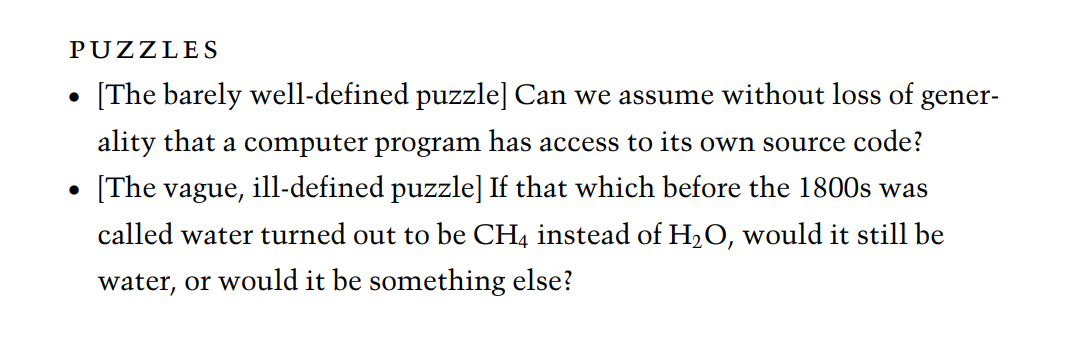
\includegraphics[angle=0, width=14cm, height=5cm]{puzzles4.png}
\end{frame}
\end{document}
